\section{Lezione dell'08/03/2018}

\subsection{Notazione asintotica}
Il \textbf{tempo di esecuzione} è difficile da calcolare, come visto nella sezione \ref{is:complessita}. 
Il modo in cui è stato calcolato è pieno di dettagli ``inutili''.\par
Rivediamo le complessità di Insertion Sort e Merge Sort:
\begin{gather*}
	T^{IS} = an^2 + bn + c \\
	T^{MS} = an \log_2 n + bn + c
\end{gather*}

A noi interessa calcolare $T(n)$ per $n$ ``grande''. Non consideriamo le costanti moltiplicative, che sono non fondamentali. Ecco una lista di possibili complessità ordinate in senso decrescente (le prime due categorie appartengono alla classe dei \emph{problemi NP}, ossia non trattabili):

\begin{itemize}[noitemsep]
	\item $3^n$
	\item $2^n$
	\medskip
	\item $n^k$
	\item $n^2$
	\item $n \log n$
	\item $n$
	\item $\log n$
	\item $1$
\end{itemize}

Prendiamo in esame due funzioni: $f(n)$, $g(n)$:

\begin{displaymath}
f, g: \mathbb{R}^+ \rightarrow \mathbb{R}^+
\end{displaymath}

\begin{itemize}
	\item $f(n)$ è la funzione in esame della complessità del nostro problema P;
	\item $g(n)$ è la funzione che, moltiplicata per un'opportuna costante $c_i$, dopo un certo $n$, fa da 
	limite superiore o inferiore per ogni punto di $f(n)$.
\end{itemize}

\subsubsection{Limite asintotico superiore}
Data $g(n)$, indichiamo con $O \big(g(n) \big)$ il \emph{limite asintotico superiore}, definito come segue:
\begin{displaymath}
	O \big(g(n) \big) = \{ f(n) \ \vert \ \exists c > 0 \quad \exists n_0 (\in \mathbb{N}) \ \vert \ \forall n \geq n_0 \Rightarrow (0 \leq) f(n) \leq c \cdot g(n) \}
\end{displaymath}

\begin{center}
	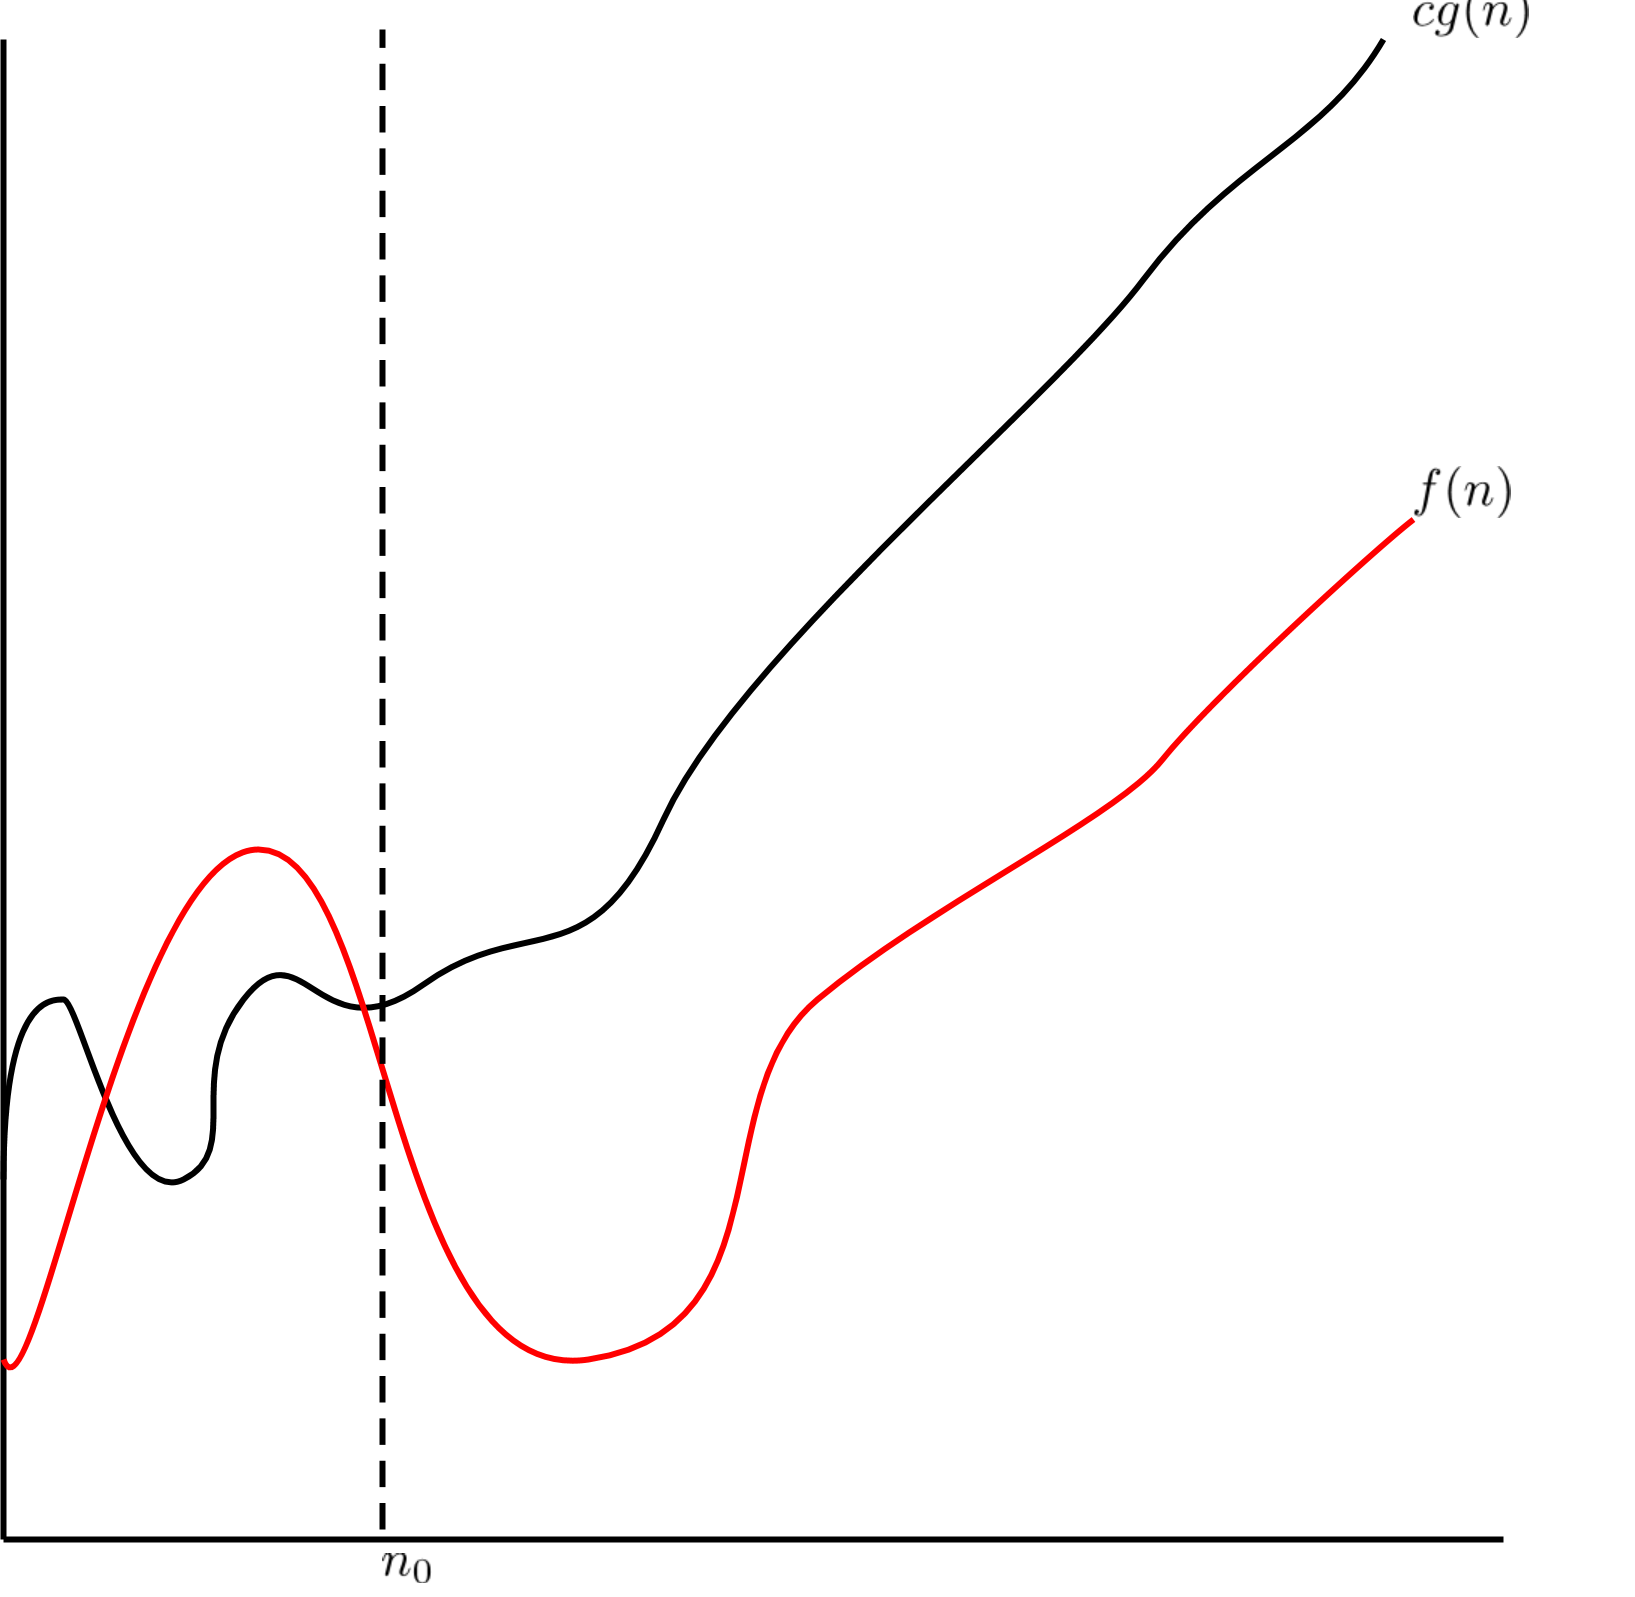
\includegraphics[width=0.80\textwidth]{img/plots/plotO.png}
\end{center}

\paragraph{Esempi}
\begin{itemize}
	\item $f_1(n) = 2n^2 + 5n + 3 = O \big(g(n^2) \big)$ ? Sì. \par
	Deve valere $f_1(n) < cn^2 \qquad \exists c > 0, \ n \geq n_0$ \par
	Ipotizziamo $c = 3$
	\begin{align*}
		2n^2 + 5n + 3 & \leq 3n^2 \\
		n^2 - 5n - 3 & \geq 0 \\
		\frac{5 \pm \sqrt{2 \cdot 5 + 12}}{2} = \frac{5 \pm \sqrt{37}}{2} \cong 5.54 && \text{(Non considero la soluzione} \\ && \text{negativa, poiché siamo in } \mathbb{R}^+ \text{)}
	\end{align*}
	\begin{center}
%		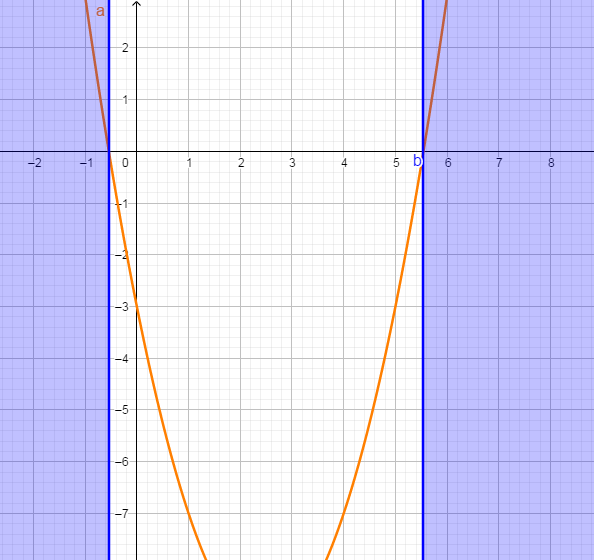
\includegraphics[height=6cm]{img/parabola-plot1.png}
	\end{center}
	
	Prendo $c = 3$ e $n_0 = 6$. Vale dunque:
	\begin{displaymath}
		f_1(n) \leq cn^2 \quad \forall n \geq n_0
	\end{displaymath}

	\item $f_1(n) = O \big(g(n^3) \big)$ ? Sì. \par
	$c = 3 $\par
	$n_0 = 6 \quad \forall n \geq n_0$ \par
	$f_1(n) \leq cn^2 \leq cn^3$
	
	\item $f_2(n) = 2 + \sin (n) = O(1)$ ? Sì. \par
	$-1 \leq \sin (n) \leq 1$ \par
	$1 \leq f_2(n) \leq 3$ \par
	Vale la seguente
	\begin{gather*}
		\exists c > 0 \quad \exists n_0 : n \geq n_0 \Rightarrow f_2(n) \leq c \cdot 1 \\
		\text{ok per } c = 3, \ n_0 = 0
	\end{gather*}
\end{itemize}

\subsubsection{Limite asintotico inferiore}
Data $g(n)$, indichiamo con $\Omega \big(g(n) \big)$ il \emph{limite asintotico inferiore}, definito come segue:
\begin{displaymath}
	\Omega \big(g(n) \big) = \{ f(n) \ \vert \ \exists c > 0 \quad \exists n_0 (\in \mathbb{N}) \ \vert \ \forall n \geq n_0 \Rightarrow c \cdot g(n) \leq f(n) \}
\end{displaymath}

\begin{center}
	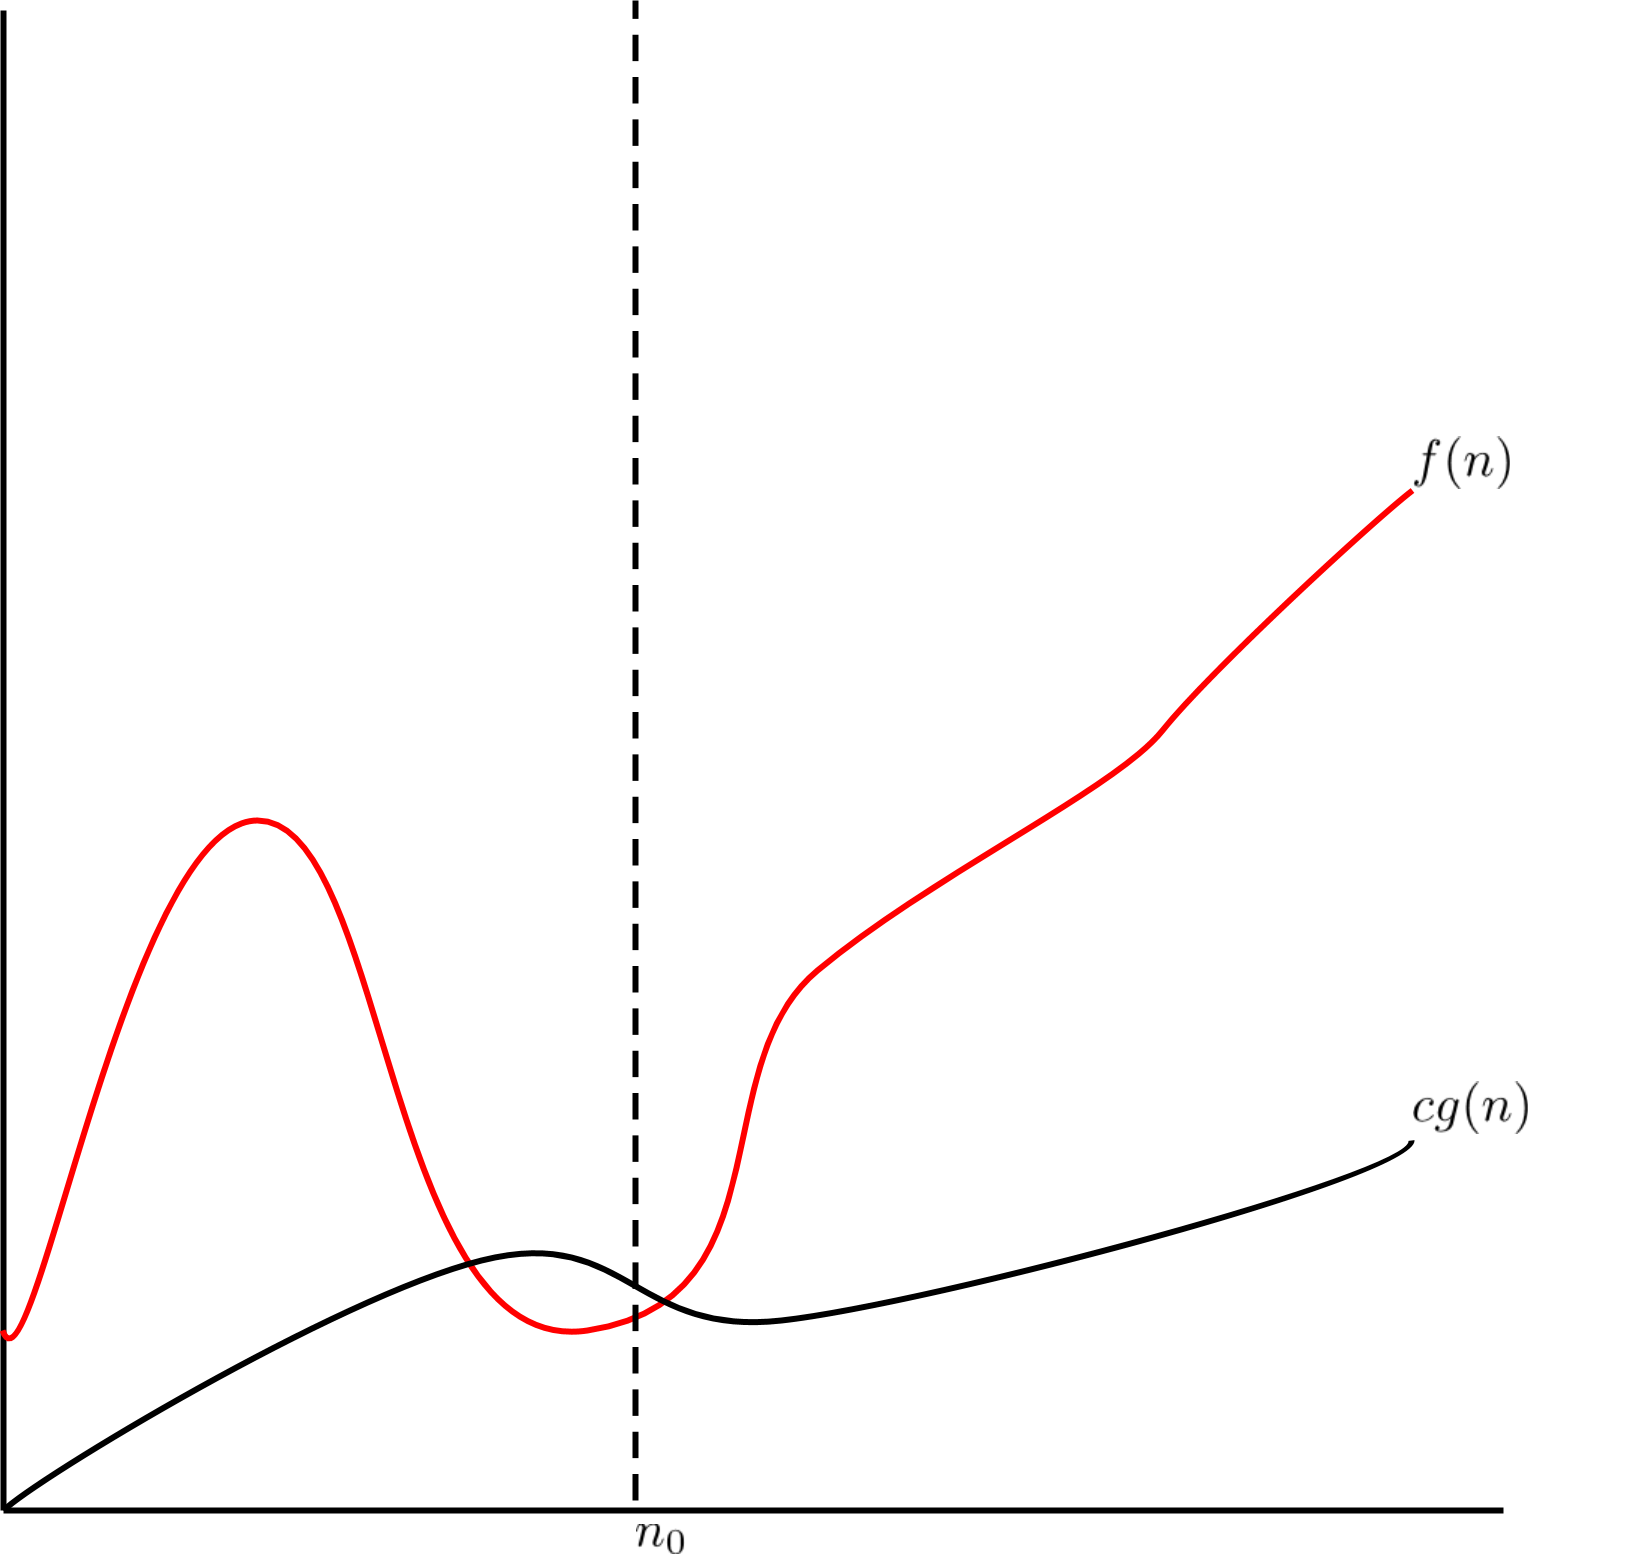
\includegraphics[width=0.80\textwidth]{img/plots/plotomega.png}
\end{center}

\paragraph{Esempi}
\begin{itemize}
	\item $f_1(n) = 2n^2 + 5n + 3 = \Omega \big(g(n^2) \big)$ ? Sì.\par
	Deve valere: \par
	\begin{displaymath}
		\exists c > 0 \quad \exists n_0 : \forall n \geq n_0 \Rightarrow cn^2 \leq 2n + 5n + 3
	\end{displaymath}
	Basta porre $c = 1$, $n_0 = 0$.
	
	\item $f_2(n) = 2 + \sin (n) = \Omega (1)$ ? Sì.
	\begin{displaymath}
		1 \leq f_2(n) \leq 3 \quad c = 1, \ n_0 = 0
	\end{displaymath}
\end{itemize}

\subsubsection{Limite asintotico stretto}
Data $g(n)$, indichiamo con $\Theta \big( g(n) \big)$ il \emph{limite asintotico stretto}, definito come segue:
\begin{multline*}
	\Theta \big( g(n) \big) = \{ f(n) \ \vert \ \exists c_1, c_2 > 0 \quad \exists n_0 (\in \mathbb{N}) \ \vert \ \forall n \geq n_0 \\ 
	\Rightarrow c_1 \cdot g(n) \leq f(n) \leq c_2 \cdot g(n) \}
\end{multline*}

\begin{center}
	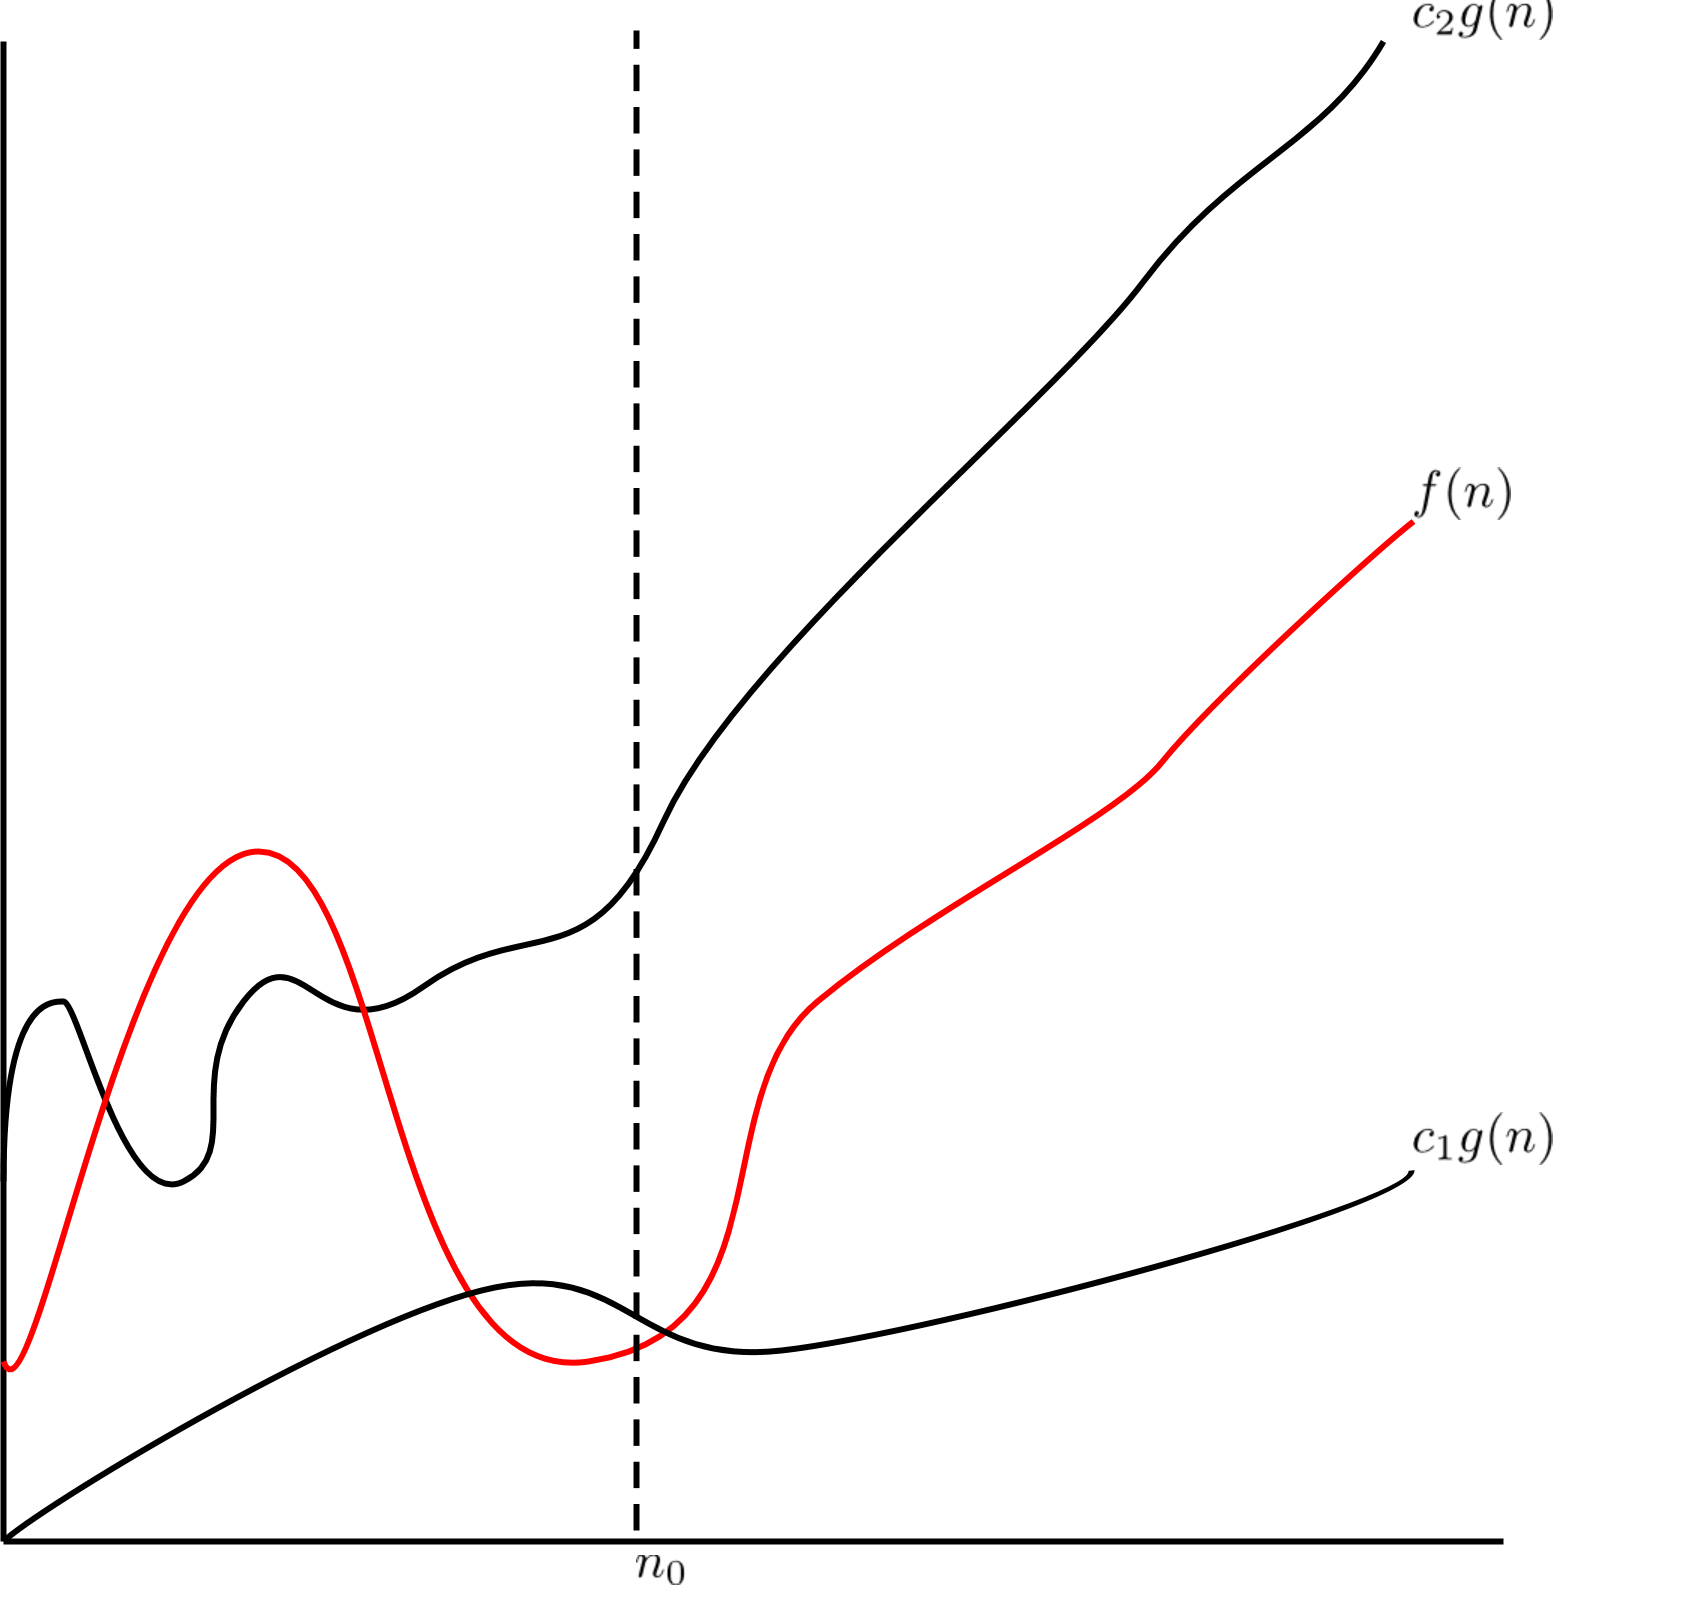
\includegraphics[width=0.80\textwidth]{img/plots/plottheta.png}
\end{center}

\paragraph{Esempi}
\begin{align*}
	f_1(n) = & 2n^2 + 5n + 3 = \Theta (n^2) && f_1(n) \neq \Theta (n^3) \\
	& c_1 = 1 \quad c_2 = 3 \quad n_0 = 6 && f_1(n) = O(n^3) \\
	f_2(n) = & 2 + \sin (n) = \Theta (1) && f_1(n) \neq \Omega (n^3) \\
	& c_1 = 1 \quad c_2 = 3 \quad n_0 = 0 && \qquad \Downarrow \\
	& && \frac{f_1(n)}{n_3} \rightarrow 0
\end{align*}

\subsection{Metodo del limite}
$f(n),g(n) > 0 \quad \forall n$ \par \medskip
Se $\lim_{n \to +\infty} \frac{f(n)}{g(n)}$ esiste, allora:

\begin{enumerate}
	\item Se $\lim_{n \to +\infty} \frac{f(n)}{g(n)} = k > 0$ allora $f(n) = \Theta \big( g(n) \big)$.\par
	\begin{align*}
		\text{Infatti } \forall \varepsilon > 0 \ \exists n_0 : \forall n \geq n_0 & \Rightarrow \abs{\frac{f(n)}{g(n)} - k} \leq \varepsilon \\
		& \Rightarrow - \varepsilon \leq \frac{f(n)}{g(n)} - k \leq \varepsilon 
	\end{align*}
	\begin{gather*}
		k - \varepsilon \leq \frac{f(n)}{g(n)} \leq k + \varepsilon \\
		(k - \varepsilon)g(n) \leq f(n) \leq (k + \varepsilon)g(n) \qquad \text{per } 0 < \varepsilon < k
	\end{gather*}
	
	\item Se $\lim_{n \to +\infty} \frac{f(n)}{g(n)} = 0$ allora $f(n) = O \big( g(n) \big)$ e 
	$f(n) \neq \Omega \big( g(n) \big)$.
	
	\item Se $\lim_{n \to +\infty} \frac{f(n)}{g(n)} = \infty$ allora $f(n) = \Omega \big( g(n) \big)$ e 
	$f(n) \neq O \big( g(n) \big)$.
\end{enumerate}

\subsection{Alcune proprietà generali}
\begin{itemize}
	\item $f(n) = a_kn^k + a_{k-1}n^{k-1} + \dots + a_1n + a_0 = \Theta (n^k)$
	\item $h \neq k \quad \Theta (n^h) \neq \Theta (n^k)$
	\item $a \neq b \quad \Theta (a^k) \neq \Theta (b^n)$
	\item $h \neq k \quad \Theta (a^{n+h}) = \Theta (a^{n+k})$
	\item $a \neq b \quad \Theta (\log_an) = \Theta (\log_bn)$
\end{itemize} 
In generale
\begin{gather*}
	O(1) \subseteq O(\log n) \subseteq O(n) \subseteq O(n \log n) \subseteq O(n^2) \subseteq \dots
\end{gather*}
Rivediamo \texttt{Insertion Sort} con le notazioni asintotiche:
\begin{displaymath}
	T^{IS}(n) = O(n^2) \qquad T^{IS}_{max}(n) = \Theta (n^2)
\end{displaymath}
Vale anche la proprietà seguente:
\begin{align*}
	2n^3 + \Theta (n^2) = O(n^3) (&\subseteq \Theta (n^3)) \\
	& = \Theta (n^3)
\end{align*}